\documentclass[tikz,border=5pt]{standalone}

\begin{document}
\setcounter{chapter}{7}
\centering
\vspace{2cm}
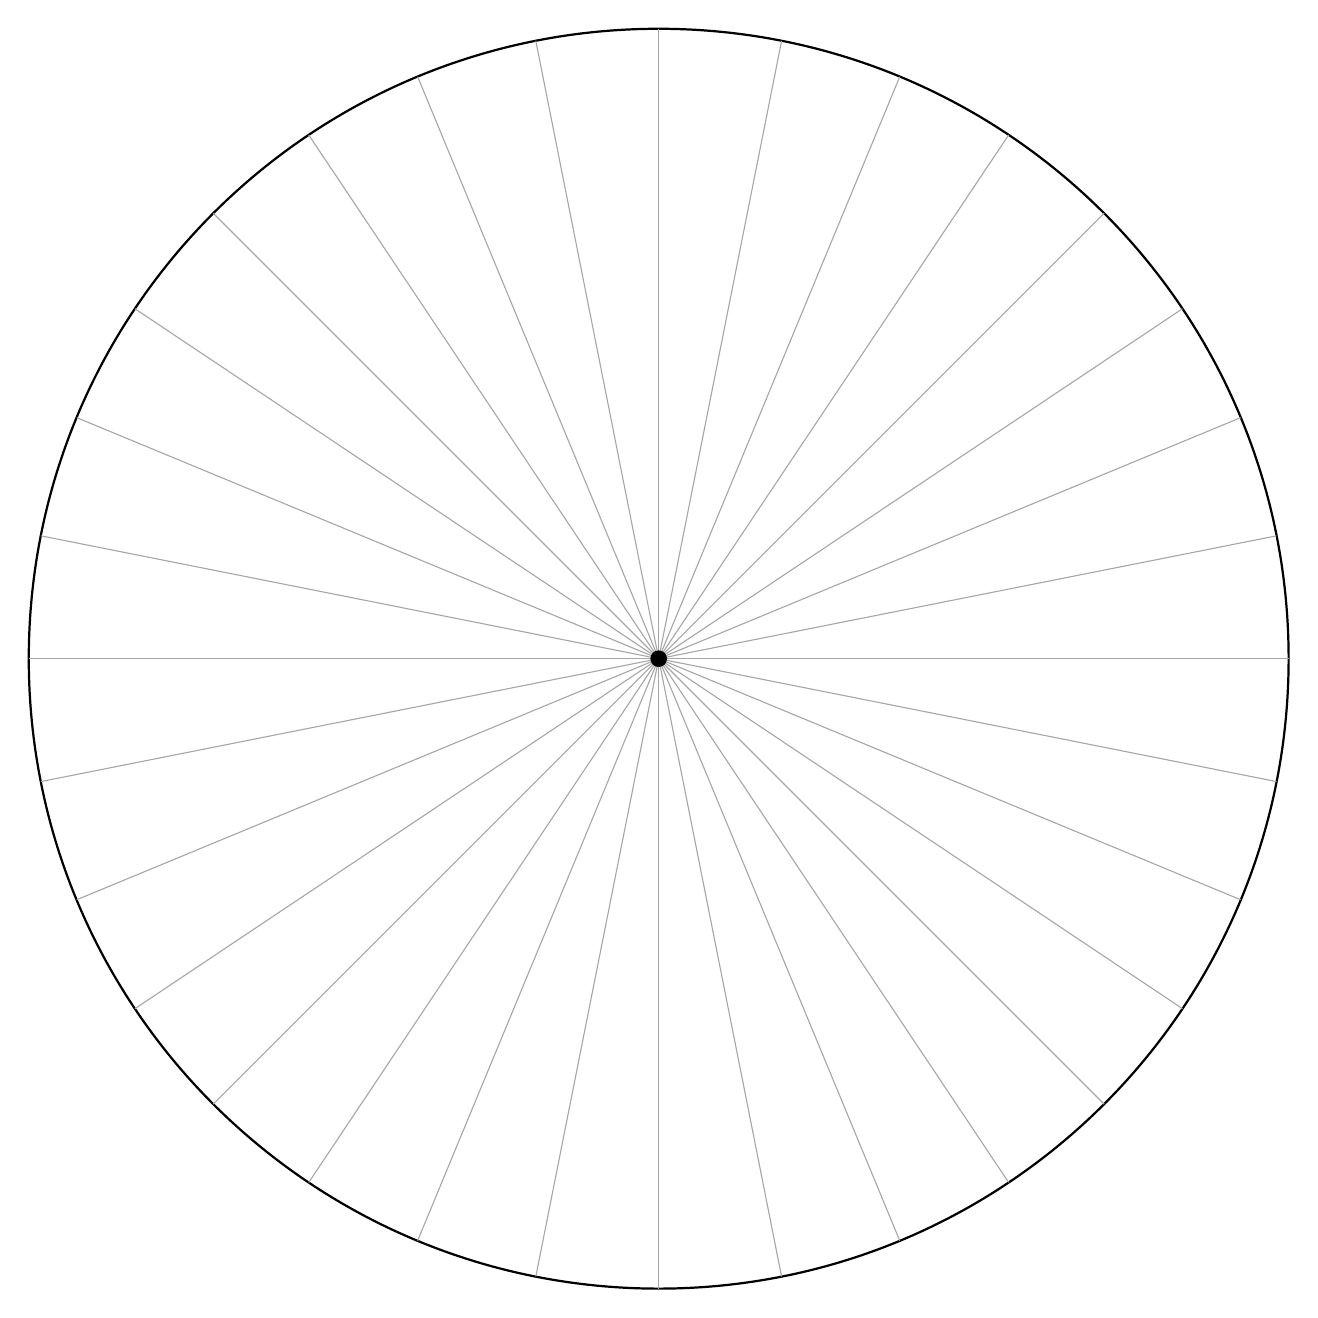
\begin{tikzpicture}[scale=2]
    % On définit le rayon du disque
    \def\radius{4}

    % Tracer le cercle extérieur
    \draw[thick] (0,0) circle (\radius);

    % Boucle pour tracer les 32 rayons
    % On divise 360 degrés par 32 = 11.25 degrés par section
    \foreach \angle in {0, 11.25, ..., 348.75} {
        \draw[thin, gray!70] (0,0) -- (\angle:\radius);
    }
    
    % Optionnel : Ajouter des points au centre pour la propreté
    \fill (0,0) circle (1.5pt);
    
\end{tikzpicture}
\end{document}